\chapter{Аналитическая часть}
В данном разделе будут рассмотрены три алгоритма сортировок: сортировка вставками и ее улучшение сортировка Шелла, сортировка выбором и ее улучшение пирамидальная сортировка и сортировка бусинами.
\section{Сортировка вставками}

Суть алгоритма заключается в следующем: на каждом  шаге  алгоритма  выбирается один  из  элементов входных данных и  помещается  на нужную  позицию  в  уже  отсортированной последовательности до тех  пор,  пока  набор  входных  данных  не будет  исчерпан.  Алгоритму  необходимо  для  каждого нового  элемента  выбрать нужное место для вставки в уже упорядоченный массив данных, так что элементы  входной  последовательности просматриваются  по одному,  и каждый новый поступивший элемент размещается  в  подходящее  место среди  ранее  упорядоченных  элементов

\subsection{Сортировка Шелла}

Метод предложен в 1959 году и назван по имени автора метода Дональда Шелла (Donald Shell). 

Сортировка Шелла \cite{book_lipachev, book_sort_algorithms, book_knut} (англ. Shell Sort) является улучшением сортировки вставками. Часто еще называемый "сортировка вставками с уменьшением расстояния". Основная идея этого метода заключается в том, чтобы в начале устранить массовый беспорядок в массиве, сравнивая далеко
отстоящие друг от друга элементы. Постепенно интервал между сравниваемыми элементами уменьшается до единицы. Это означает, что на поздних стадиях сортировка сводится просто к перестановкам соседних элементов (если, конечно, такие перестановки являются необходимыми).

Пусть $d$ - интервал между сравниваемыми элементами. Первоначально используемая Шеллом последовательность длин промежутков: $d_1 = \frac{N}{2}, d_{i} = \frac{d_{i - 1}}{2}, … d_k = 1$. Процесс завершается обычной сортировкой вставками получившегося списка.

\section{Сортировка выбором}

Алгоритм сортировки выбором заключается в поиске на необработанном срезе массива или списка минимального значения и в дальнейшем обмене этого значения с первым элементом необработанного среза. На следующем шаге необработанный срез уменьшается на один элемент.

Шаги выполнения алгоритма:
\begin{enumerate} 
	\item Находим  минимальный (максимальный)  элемент  в  текущем  массиве. 
	\item Производим обмен этого элемента со значением первой неотсортированной позиции.  Обмен  не  нужен,  если минимальный (максимальный) элемент уже находится на данной позиции. 
	\item Сортируем оставшуюся часть массива, исключив из рассмотрения уже отсортированные элементы. 
\end{enumerate}

\subsection{Пирамидальная сортировка}

Пирамидальная сортировка \cite{book_lipachev, book_sort_algorithms, book_knut, book_kormen}  (англ. Heap Sort) предложена в 1964 году Дж. Уильямсом. Основана на использовании бинарного сортирующего дерева (пирамиды) и базируется на сортировке выбором, по сути является его усовершенствованием.

Пирамида (англ. binary heap) определяется как структура данных, представляющая собой объект-массив, который можно рассматривать как почти полное бинарное дерево. Каждый узел этого дерева соответствует определенному элементу массива. На всех уровнях, кроме, может быть, последнего, дерево полностью заполнено (заполненным считается уровень, который содержит максимально возможное количество узлов). Последний уровень заполняется слева направо до тех пор, пока в массиве не закончатся элементы. 

В пирамиде, представленной на рисунке \ref{fig:heap_structs}, число в окружности, представляющей каждый узел дерева, является значением, сортируемым в данном узле. Число над узлом — это соответствующий индекс массива. Линии, попарно соединяющие элементы массива, обозначают взаимосвязь вида “родитель-потомок”. Родительские элементы всегда расположены слева от дочерних. Данное дерево имеет высоту, равную 3; узел с индексом 4 (и значением 8) расположен на первом уровне.

\begin{figure}[h]
	\centering
	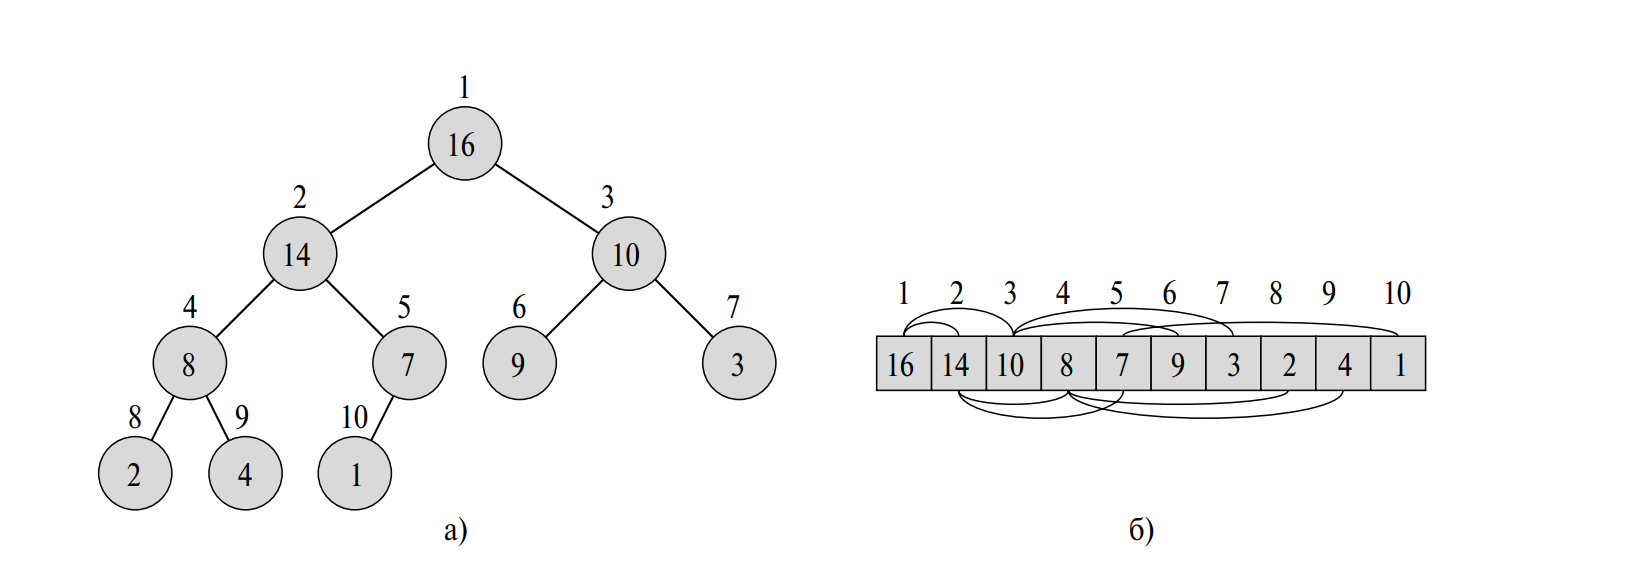
\includegraphics[height=0.25\textheight]{img/heap_structs.png}
	\caption{Пирамида, представленная в виде a) бинарного дерева и б) массива}
	\label{fig:heap_structs}
\end{figure}

Обозначим, что:
\begin{enumerate} 
	\item Родительский элемент в массиве будет находится под индексом - $\frac{i}{2}$;
	\item Правый потомок в массиве будет находится под индексом - $2 \cdot i$;
	\item Левый потомок в массиве будет находится под индексом - $2 \cdot i + 1$.
\end{enumerate}

Различают два вида бинарных пирамид: неубывающие и невозрастающие. В пирамидах обоих видов значения, расположенные в узлах, удовлетворяют свойству пирамиды (heap property), являющемуся отличительной чертой пирамиды того или иного вида. Свойство невозрастающих пирамид (max-heap property) заключается в том, что для каждого отличного от корневого узла с индексом $i$ выполняется следующее неравенство

\begin{equation}
	A[i / 2] \geq A[i]
\end{equation}

Другими словами, значение узла не превышает значение родительского по отношению к нему узла. Таким образом, в невозрастающей пирамиде самый большой элемент находится в корне дерева, а значения узлов поддерева, берущего начало в каком-то элементе, не превышают значения самого этого элемента. Принцип организации неубывающей пирамиды (min-heap) прямо противоположный. Свойство неубывающих пирамид (min-heap property) заключается в том, что для всех отличных от корневого узлов с индексом $i$ выполняется такое неравенство:

\begin{equation}
	A[i / 2] \leq A[i]
\end{equation}

Таким образом, наименьший элемент такой пирамиды находится в ее корне.

\section{Сортировка бусинами}

Гравитационная сортировка, также известная как сортировка бусинами (англ. Bead Sort) — алгоритм сортировки, разработанный Джошуа Аруланандхамом, Кристияном Калюдом и Майклом Диннином в 2002 году.

Прародителем счётов в Европе является абак, который из Вавилона перекочевал в Египет, оттуда – в Грецию, из неё – в Рим, из которого – по всей Европе. Внешний вид и принцип действия античного «калькулятора» настолько напоминает поведение этой «простой» сортировки, что её иногда так и называют — «Абаковая сортировка» (Abacus sort).

Предположим, нужно отсортировать набор натуральных чисел. Друг под другом каждое число выложим в виде горизонтального ряда из соответствующего количества шариков. А теперь поглядим на все эти группировки шариков не по горизонталям, а по вертикалям. Сдвинем шарики вниз до упора. Снова переключимся на горизонтали и пересчитаем бусинки в каждом ряду. Получили первоначальный набор чисел, только упорядоченный.

Метод ограничен, прежде всего применим к натуральным числам, т.е. можно сортировать только положительные числа. Можно сортировать и целые, но это запутаннее - отрицательные числа придется обрабатывать отдельно отрицательные от положительных.

\section*{Вывод}
В данном разделе были рассмотрены алгоритмы сортировки - бусинами, пирамидальная и Шелла и рассмотрены некоторые их неусовершенствованные сортировки, а именно сортировка вставками и выбором. Рассмотренные сортировки следует реализовать, изучить трудоемкость и проанализировать время и память для выполнения.